% !TeX spellcheck = pl_PL
\documentclass[a4paper, 11pt]{article}
\usepackage[margin=2cm]{geometry}
\usepackage[T1]{fontenc}
\usepackage[utf8]{inputenc}
\usepackage{palatino}
\usepackage{mathpazo}
\usepackage{footnote}
\usepackage[hyphens]{url}
\usepackage{hyperref}
\usepackage[bottom]{footmisc}
\hypersetup{colorlinks, linkcolor=black, linktoc=all, urlcolor=black}
\urlstyle{rm}
\usepackage{float}
\usepackage{polski, indentfirst}
\usepackage{enumerate}
\renewcommand{\arraystretch}{1.3} % linespacing for tables

\usepackage{setspace} \onehalfspacing % document line-spacing
\usepackage{enumitem} \setlist{nolistsep} % better enumeration
\usepackage{graphicx}
\usepackage{tikz}
\usetikzlibrary{arrows,shapes.geometric}
\usepackage{verbatim}
\usepackage{longtable}
\usepackage{booktabs}

\usepackage{lscape}
\usepackage{ifxetex}
\ifxetex
\usepackage{fontspec}
\usepackage{xunicode}
\setmainfont{TeX Gyre Pagella}
\else
\fi


\begin{document}
	
	\noindent
\begin{minipage}[t]{.5\linewidth}
	\begin{flushleft}
		Grupa projektowa: \tabto{3.5cm}\textbf{WT 9:15}\\
		\vspace{0.8cm}
		Piotr Chmiel \tabto{3.5cm}200608\\
		Kamil Machnicki \tabto{3.5cm}200752\\
		Łukasz Matysiak \tabto{3.5cm}200646\\
		Michał Polański \tabto{3.5cm}200852\\
		Maciej Stelmaszuk \tabto{3.5cm}200654\\
		Jakub Zgraja \tabto{3.5cm}200609\\
	\end{flushleft} 
\end{minipage}%
\begin{minipage}[t]{.5\linewidth}
	\begin{flushright}
		Wrocław, {\today} r.\\
		\vspace{.35cm}

	\end{flushright}
\end{minipage}

\vspace{3.0cm}

\begin{center}
	{\Huge\bf Deeplearning -- tagger}\\
	{\Large\bf (POS, lematyzacja)}\\
		
	\bigskip{\Large \uppercase{DOKUMENTACJA PROJEKTOWA}}
\end{center}

\begin{center}
	{\large Kurs ,,Zastosowania informatyki w gospodarce''}\\
	{\large Rok akad. 2015/2016, kierunek INF, studia II stopnia}
\end{center}

\vspace{2cm}
\begin{center}
		\textsc{Prowadzący:}\\
		dr inż. Tomasz Walkowiak
\end{center}

	\thispagestyle{empty}
	
	\newpage
	\tableofcontents
	
	\newpage
	\section{Cel projektu}

\textbf{Temat projektu:} {\large \textit{Deeplearning -- tagger (POS, lematyzacja)}.}
\medskip

Zadaniem realizowanego przedsięwzięcia jest stworzenie programu głębokiego uczenia (ang. \textit{deep learning}) z zakresu przetwarzania języka naturalnego. Jego celem jest przypisywanie każdemu wyrazowi w tekście wejściowym odpowiadającej mu części mowy (ang. \textit{part-of-speech, POS}). Wykonanie zadania tagowania zostanie poprzedzone procesem lematyzacji tekstu.


\begin{figure}[H]
	\centering
	\begin{tikzpicture}[node distance=3cm,auto,>=latex']
		\tikzstyle{box} = [rectangle, draw, fill=blue!10, rounded corners, inner sep=.5em]
		\tikzstyle{ball} = [ellipse, draw, fill=blue!10, align=center, anchor=north, inner sep=.5em]
		\node (a) {\textit{,,Ala ma kota''}};
		\node (b) [box, right of=a, node distance=3.5cm] {lematyzator};
		\node (c) [box, right of=b, node distance=5.5cm] {POS tagger};
		\node (d) [right of=c, node distance=3.8cm] {
			\tabcolsep=1.5pt
			\renewcommand{\arraystretch}{1}
			\begin{tabular}{ccc}
				{\footnotesize RZ} & {\footnotesize CZ} & {\footnotesize RZ} \\
				\textit{,,Ala} & \textit{mieć} & \textit{kot''}
			\end{tabular}
		};
		\node (c1) [box, above of=c, node distance=2cm] {lematyzator};
		\node (c2) [ball, above of=c1, node distance=1.5cm] {zbiór uczący};
		\path[->] (a) edge node {} (b);
		\path[->] (b) edge node {\textit{,,Ala mieć kot''}} (c);
		\draw[->] (c) edge node {} (d);
		\draw[->] (c1) edge node [anchor=center,fill=white]{uczenie} (c);
		\draw[->] (c2) edge node {} (c1);
	\end{tikzpicture}
	\caption{Uproszczony schemat działania programu.}
\end{figure}

Realizacja powinna posiadać formę aplikacji desktopowej lub skryptu. Cel projektu zostanie osiągnięty, jeśli przygotowane oprogramowanie (wyposażone w odpowiedni zbiór uczący) będzie w stanie przetwarzać tekst w języku polskim w czasie i dokładności, które zostaną sprecyzowane przez prowadzącego.


\section{Koszty}
\subsection*{Szacunkowy czas wykonania}
Biorąc pod uwagę zakres tematyczny projektu szacuję się, że do jego wykonania potrzebnych jest 400 godzin roboczych. Około 1/8 czasu poświęcone będzie na zebranie i analizę materiałów dotyczących projektu, ogólne poznanie możliwości i technologii. Największa część czasu zużyta zostanie na implementację projektu (stworzenie lematyzatora oraz taggera). Szacuje się, że będzie to 6/8 czasu. Pozostała część przeznaczona jest na kontakty z prowadzącym oraz testy zaimplementowanego rozwiązania.

\subsection*{Szacunkowy koszt projektu}
Mając na uwadze poziom skomplikowania zadania projektowego stawka za godzinę pracy wynosi 150 zł. Przy szacowaniu kosztów projektu nie uwzględniamy dodatkowych wydatków, które trzeba będzie ponieść w przypadku, gdy np. zajdzie potrzeba wykupienia domeny WWW. Nie są uwzględnione także koszty wdrożenia projektu w środowisku produkcyjnym. W związku z powyższym szacunkowy koszt wykonania projektu jest równy 60 000 zł netto.

Usługi, o których mowa w poprzednich punktach opodatkowane są 23\% stawką podatku VAT (podatek od towarów i usług). Szacowana cena brutto wynosi \textbf{73 800 zł}.

\begin{table}[H]
	\centering
	\caption{Kosztorys.}
	\smallskip
	\begin{tabular}{cccccccc}
		\toprule
		\textbf{Nazwa} & \textbf{Jedn.} & \textbf{Ilość} & \textbf{Cena jedn.} & \textbf{Wart. netto} & \textbf{Stawka} & \textbf{Podatek} & \textbf{Wart. brutto} \\
		\midrule
		Robocizna & r-g & 400 & 150 zł & 60 000 zł & 23\% & 13 800 zł & 73 800 zł \\
		\bottomrule
		\multicolumn{7}{r}{\bf Razem:} & \textbf{73 800 zł} \\
	\end{tabular}
\end{table}

\section{Terminy i harmonogram projektu}
Granicznym terminem realizacji projektu jest \textbf{7 czerwca 2016 r}. W tym dniu nastąpi prezentacja rezultatów projektu wraz z przekazaniem jego pełnej dokumentacji.

\begin{table}[H]
	\centering
	\caption{Harmonogram projektu.}
	\smallskip
	\begin{tabular}{p{4cm}p{8cm}}
		\toprule
		\textbf{Data}& \textbf{Opis} \\
		\midrule
		23.02.2016 & Wybór tematu projektu. \\
		1.03.2016 & Określenie zakresu tematycznego projektu. \\
		8.03.2016 & Przekazanie specyfikacji projektu (wstępna funkcjonalność, określenie kamieni milowych). \\
		9.03.2016 -- 06.06.2016 & Konsultacja wyników pracy po osiągnięciu kolejnych kamieni milowych projektu. \\
		7.06.2016 & Prezentacja rezultatów projektu i przekazanie dokumentacji projektowej. \\
		\bottomrule
	\end{tabular}
\end{table}

	\begin{table}[H]
	\centering
	\caption{Kamienie milowe.}
	\smallskip
	\begin{tabular}{p{4cm}p{8cm}}
		\toprule
		\textbf{Data}& \textbf{Opis} \\
		\midrule
		29.03.2016 & Instalacja środowiska \\
		19.04.2016 & Stworzenie lematyzatora \\
		10.05.2016 & Stworzenie taggera \\
		31.05.2016 & Stworzenie instrukcji użytkowania \\
		07.06.2016 & Prezentacja projektu \\
		\bottomrule
	\end{tabular}
\end{table}

	\input{app-docs}
	\section{Przetwarzanie danych}
	\subsection{Konwersja plików XML do formatu CSV}
	Ze względu na nieefektywność przetwarzania plików XML oraz na dużą ilość niepotrzebnych danych znajdujących się w korpusach, postanowiono przetworzyć je do formy plików CSV.
Proces zamiany plików XML odbywa się dla obydwu korpusów -- PWr oraz podkorpusu milionowego.
	Niestety, ze względu na rozbieżność struktur nie mogą one być przetworzone w ten sam sposób.
	
\begin{sloppypar}
Do pliku CSV zapisywane są dwie informacje -- słowo oraz część mowy.
Wyrażenia XPath służące do wydobycia tych danych z korpusu PWr wyglądają następująco:
\texttt{//tok/orth} -- dla wyrazu, oraz \texttt{//tok/lex[disamb='1']} dla części mowy. Dla podkorpusu milionowego zapytania XPath prezentują się w sposób następujący: \texttt{//f[name='orth']/string} dla wyrazu, oraz \texttt{//f[name='disamb']/f[name='interpretation']/string} dla części mowy.
\end{sloppypar}

	\subsection{Mapowanie klas NKJP}
Oba korpusy wykorzystują zestaw znaczników morfosyntaktycznych NKJP, który wyróżnia 36 rodzajów klas.
Na potrzeby projektu liczba ta została ograniczona do 10 podstawowych części mowy. Poniżej zostało przedstawione mapowanie z klas NKJP na uproszczony model.
\begin{table}[H]
	\centering
	\caption{Mapowanie klas NKJP.}
	\begin{tabular}{p{3cm}p{.5cm}p{11cm}}
		\toprule
		\texttt{rzeczownik} & $\leftarrow$ & rzeczownik, rzeczownik deprecjatywny. \\
		\texttt{liczebnik} & $\leftarrow$ & liczebnik główny, liczebnik zbiorowy. \\
		\texttt{przymiotnik} & $\leftarrow$ & przymiotnik, przymiotnik przyprzym., przymiotnik poprzyimkowy, przymiotnik predykatywny. \\
		\texttt{przysłówek} & $\leftarrow$ & przysłówek. \\
		\texttt{zaimek} & $\leftarrow$ & zaimek nietrzecioosobowy, zaimek trzecioosobowy, zaimek siebie. \\
		\texttt{czasownik} & $\leftarrow$ & forma nieprzeszła, forma przyszła być, aglutynant być, pseudoimiesłów, rozkaźnik, bezosobnik, bezokolicznik, im. przys. współczesny, im. przys. uprzedni, odsłownik, im. przym. czynny, im. przym. biern, winien, predykatyw. \\
		\texttt{przyimek} & $\leftarrow$ & przyimek, wykrzyknik. \\
		\texttt{spójnik} & $\leftarrow$ & spójnik współrzędny, spójnik podrzędny. \\
		\texttt{partykuła} & $\leftarrow$ & kublik. \\
		\texttt{forma nierozpoznana} & $\leftarrow$ & skrót, burkinostka, interpunkcja, ciało obce, forma nierozpoznana. \\
		\bottomrule
	\end{tabular}
\end{table}

\section{Opis danych}
	System operuje na danych wejściowych, którymi są słowa w języku polskim.
	Istnieje możliwość wprowadzenia zarówno pojedynczego słowa, jak i wielu (np. epitety, całe zdania).
	
	\subsection{Sposób wybierania cech}
	Cechy wybierane są na podstawie budowy słowa oraz kontekstu, w którym zostało użyte.
	W celu wyekstrahowania cech ze słowa, system bada $N$ ostatnich liter wyrazu oraz to, jakie części zdania wystąpiły wcześniej.
	
	W zależności od wyboru użytkownika, system potrafi zebrać dane uczące z korpusu PWr lub z korpusu podmilionowego.
	
	\subsubsection{Zaimplementowana metoda wybierania cech}
	Metoda ekstrakcji cech zaimplementowana w systemie opiera się na wyodrębnianiu końcówek wyrazów.
	
	Możliwe jest wybranie od jednej do czterech ostatnich liter, z których następnie jest tworzona macierz cech -- wybierane są najczęściej występujące końcówki, wraz z etykietą, którą część mowy stanowią.
	
	Liczba najczęściej występujących końcówek zależy od ich długości:
	\begin{itemize}
		\item 15 najczęstszych końcówek jednoliterowych,
		\item 35 najczęstszych końcówek mających od dwóch do czterech liter.
	\end{itemize}
	
	Oprócz końcówek wyrazów, dla zdań występujących w korpusach, podawane są etykiety poprzednich dwóch wyrazów.
	
	\subsubsection{Przykład macierzy cech}
	Przykładowy zbiór uczący:
	\begin{itemize}
		\item jabłkami -- rzeczownik,
		\item niepoważny -- przymiotnik,
		\item kierunku -- rzeczownik,
		\item istnieje -- czasownik,
		\item wolność -- rzeczownik,
	\end{itemize}
	
	\medskip
	Podane wyrazy nie posiadają danych na temat poprzednich etykiet wyrazów. Można wyróżnić tutaj następujące końcówki:
	\begin{itemize}
		\item i -- rzeczownik,
		\item y -- przymiotnik,
		\item u -- rzeczownik,
		\item e -- czasownik,
		\item ć -- rzeczownik,
		\item mi -- rzeczownik,
		\item ny -- przymiotnik,
		\item ku -- rzeczownik,
		\item je -- czasownik,
		\item ść -- rzeczownik,
		\item ami -- rzeczownik,
		\item żny -- przymiotnik,
		\item nku -- rzeczownik,
		\item eje -- czasownik,
		\item ość -- rzeczownik,
		\item kami -- rzeczownik,
		\item ażny -- przymiotnik,
		\item unku -- rzeczownik,
		\item ieje -- czasownik,
		\item ność -- rzeczownik.
	\end{itemize}
	
	\medskip
	Etykiety są zamieniane na format wykorzystywany przez pakiet \texttt{scikit-learn} przy pomocy klasy \texttt{DictVectorizer}:
	\begin{itemize}
		\item rzeczownik $\rightarrow$ 0
		\item przymiotnik $\rightarrow$ 1
		\item czasownik $\rightarrow$ 2
		\item --- (b.d.) $\rightarrow$ 3
	\end{itemize}
	
	\begin{landscape}
	\newcommand{\hl}[1]{\colorbox{black!20!white}{#1}}
	\noindent Dla podanego zbioru uczącego można wyróżnić macierz cech (końcówki liter $\rightarrow$ czy dany wyraz kończy się na daną końcówkę):
	\begin{table}[H]
	\caption{Przykładowa macierz cech.}
	\footnotesize
	%\hskip-1.2cm
	\centering
	\begin{tabular}{l|cccccccccccccccccccc|ccc}
	\toprule
	& i & y & u & e & ć & mi & ny & ku & je & ść & ami & żny & nku & eje & ość & kami & ażny & unku & ieje & ność & etykieta w. n-1 & etykieta w. n-2 & etykieta \\
	\midrule
	jabłkami & \hl{1} & 0 & 0 & 0 & 0 & \hl{1} & 0 & 0 & 0 & 0 & \hl{1} & 0 & 0 & 0 & 0 & \hl{1} & 0 & 0 & 0 & 0 & 3 & 3 & 0 \\
	niepoważny & 0 & \hl{1} & 0 & 0 & 0 & 0 & \hl{1} & 0 & 0 & 0 & 0 & \hl{1} & 0 & 0 & 0 & 0 & \hl{1} & 0 & 0 & 0 & 3 & 3 & 1 \\
	kierunku & 0 & 0 & \hl{1} & 0 & 0 & 0 & 0 & \hl{1} & 0 & 0 & 0 & 0 & \hl{1} & 0 & 0 & 0 & 0 & \hl{1} & 0 & 0 & 3 & 3 & 0 \\
	istnieje & 0 & 0 & 0 & \hl{1} & 0 & 0 & 0 & 0 & \hl{1} & 0 & 0 & 0 & 0 & \hl{1} & 0 & 0 & 0 & 0 & \hl{1} & 0 & 3 & 3 & 2 \\
	wolność & 0 & 0 & 0 & 0 & \hl{1} & 0 & 0 & 0 & 0 & \hl{1} & 0 & 0 & 0 & 0 & \hl{1} & 0 & 0 & 0 & 0 & \hl{1} & 3 & 3 & 0 \\
	\bottomrule
	\end{tabular}
	\end{table}
	\normalsize
	Legenda:\\
	\begin{tabular}{lcl}
		\colorbox{white}{0} & -- & brak danej cechy w obiekcie \\
		\hl{1} & -- & dana cecha występuje dla obiektu \\
	\end{tabular}
	\end{landscape}
	
	\subsection{Wykorzystane klasyfikatory}
	Projekt wykorzystuje wiele klasyfikatorów. Wszystkie klasyfikatory z pakietu \texttt{scikit-learn} podczas procesu uczenia używają domyślnych parametrów. Więcej informacji można uzyskać w dokumentacji pakietu, dostępnej pod adresem: \url{http://scikit-learn.org/stable/modules/classes.html}.
	
	\begin{table}[H]
		\centering
		\caption{Wykorzystane klasyfikatory.}
		\begin{tabular}{p{5cm}p{11cm}}
			\toprule
			\textbf{Nazwa} & \textbf{Opis} \\
			\midrule
			\texttt{DecisionTreeClassifier} & Klasyfikator oparty na drzewie decyzyjnym. \\
			\texttt{SGDClassifier} & Klasyfikator oparty na liniowym modelu z metodą stochastycznego gradientu prostego. \\
			\texttt{SVM} & Klasyfikator reprezentuje model maszyny wektorów nośnych. \\
			\texttt{LogisticRegression} & Klasyfikator oparty na regresji logistycznej. \\
			\texttt{BernoulliNB} & Klasyfikator wykorzystujący model naiwnego klasyfikatora bayesowskiego z rozkładem Bernoulliego. \\
			\texttt{KNeighborsClassifier} & Klasyfikator implementujący mechanizm $k$-najbliższych sąsiadów. \\
			Sieć neuronowa & Klasyfikator wykorzystujący sieć neuronową opartą na bibliotece \texttt{sknn}. Posiada dwie warstwy: \texttt{Rectifier} (z liczbą 100 neuronów) i \texttt{Softmax}. Współczynnik uczenia wynosi 0.01, a liczba iteracji wynosi 10. Rectifier jest funkcją aktywacji sieci neuronowej, którą można przedstawić jako $f(x)=max(0,x)$. Dzięki takiej funkcji aktywacji można uprościć model zachowując skuteczność klasyfikacji.\\
			Sieć neuronowa wykorzystująca kartę graficzną & klasyfikator, podobnie jak powyższy wykorzystuje sieć neuronową, jednakże do implementacji wykorzystano bibliotekę \texttt{TensorFlow}, ponieważ wspiera wykorzystanie karty graficznej. Podobnie jak w poprzednim klasyfikatorze, sieć ta posiada dwie warstwy -- \texttt{Gated Recurrent Unit} z liczbą 50 neuronów oraz warstwę regresji logistycznej, współczynnik uczenia również wynosi 0.01, liczba iteracji wynosi 1000. Klasyfikator wykorzystuje klasę biblioteki \texttt{TensorFlow} -- \texttt{tf.nn.rnn} -- rekurencyjną sieć neuronową. W odróżnieniu od konwencjonalnych sieci neuronowych, rekurencyjne sieci posiadają pętle, dzięki czemu mogą wykorzystać dane z poprzednich zdarzeń podczas klasyfikacji. Taką sieć można zaprezentować jako wiele kopii tej samej sieci neuronowej, które przekazują klasyfikacje kolejnym kopiom. Ze względu na ograniczoną pamięć kart graficznych, dane uczące dzielone są na części, domyślnie po dziesięć tysięcy próbek. \\
			\bottomrule
		\end{tabular}
	\end{table}
	
	Parametry sieci neuronowych zostały dobrane empirycznie, powstały jako wynik wielu godzin eksperymentów, których celem była jak najwyższa skuteczność klasyfikowania części mowy.

	\section{Wyniki pomiarów działania programu}
\subsection{Dokładność modeli w bazie}
Badania przeprowadzono dla różnych liczb n-literowych końcówek wyrazów. Aby lepiej zobrazować otrzymane wyniki użyto notacji (\textit{liczba 1 literowych końcówek, liczba 2 literowych końcówek, liczba 3 literowych końcówek, liczba 4 literowych końcówek}).
\begin{landscape}
	\begin{table}[!htbp]
		\centering
		\caption{Skuteczność modeli -- Korpus PWr}
		\begin{tabular}{cccccccc}
			\hline
			\multicolumn{1}{|c|}{\textbf{Algorytm}} & \textbf{(15, 35, 35, 35)} & \textbf{(20, 35, 35, 35)} & \textbf{(25, 38, 38, 38)} & \textbf{(25, 40, 40, 40)} & \textbf{(28, 42, 42, 42)} & \textbf{(28, 45, 45, 45)} & \textbf{(32, 45, 45, 45)} \\ \hline
			Support Vector Machine & 56,46 & 57,46 & 58,75 & 60,03 & 61,01 & 59,94 & 58,68 \\
			Decision Trees & 57,24 & 58,12 & 59,30 & 59,97 & 60,58 & 59,10 & 58,14 \\
			Stochastic Gradient Descent & 53,62 & 54,48 & 55,37 & 56,58 & 57,72 & 56,22 & 54,97 \\
			Logistic Regression & 55,57 & 56,68 & 57,93 & 58,82 & 59,93 & 58,79 & 57,84 \\
			Naive Bayes & 54,14 & 55,42 & 56,69 & 57,72 & 58,89 & 57,58 & 56,56 \\
			K Neighbors & 50,17 & 51,35 & 52,18 & 53,30 & 54,22 & 53,12 & 52,20 \\
			Neural Networks & 55,80 & 57,08 & 57,91 & 58,88 & 60,04 & 58,72 & 57,75 \\ 
			Klasyfikator GPU & 56,24 & 57,46 & 58,34 & 59,23 & 60,51 & 59,1 & 58,22 \\ \hline
		\end{tabular}
	\end{table}
	
	\begin{table}[!htbp]
		\centering
		\caption{Skuteczność modeli -- Korpus National}
		\begin{tabular}{cccccccc}
			\hline
			\multicolumn{1}{|c|}{\textbf{Algorytm}} & \textbf{(15, 35, 35, 35)} & \textbf{(20, 35, 35, 35)} & \textbf{(25, 38, 38, 38)} & \textbf{(25, 40, 40, 40)} & \textbf{(28, 42, 42, 42)} & \textbf{(28, 45, 45, 45)} & \textbf{(32, 45, 45, 45)} \\ \hline
			Support Vector Machine & 55,43 & 56,26 & 57,63 & 59,05 & 60,13 & 59,07 & 57,55 \\
			Decision Trees & 56,04 & 57,03 & 58,25 & 59,10 & 59,38 & 57,97 & 57,15 \\
			Stochastic Gradient Descent & 53,56 & 54,35 & 55,30 & 56,53 & 57,62 & 56,16 & 54,85 \\
			Logistic Regression & 55,48 & 56,55 & 57,82 & 58,76 & 59,86 & 58,64 & 57,77 \\
			Naive Bayes & 53,11 & 54,28 & 55,70 & 56,61 & 58,06 & 56,59 & 55,39 \\
			K Neighbors & 50,02 & 51,29 & 52,03 & 53,25 & 54,13 & 53,00 & 52,08 \\
			Neural Networks & 54,69 & 56,17 & 56,95 & 57,81 & 58,87 & 57,73 & 56,77 \\
			Klasyfikator GPU & 56,04 & 57,3 & 58,02 & 58,93 & 60,22 & 58,88 & 57,96 \\ \hline 
		\end{tabular}
	\end{table}
\end{landscape}

Najlepszym klasyfikatorem okazał się być Support Vector Machine, a najgorszym K Neighbors. Konfiguracje końcówek, w których liczba dwu i więcej literowych końcówek była mniejsza niż 35 nie dawały satysfakcjonujących rezultatów. (co najmniej 50\% skuteczności) Dla konfiguracji, w których liczba tych końcówek przekracza 42 zauważono trend ku obniżaniu się skuteczności klasyfikacji dlatego też zaprzestano dalszych badań.

\begin{figure}[!htbp]
	\centering
	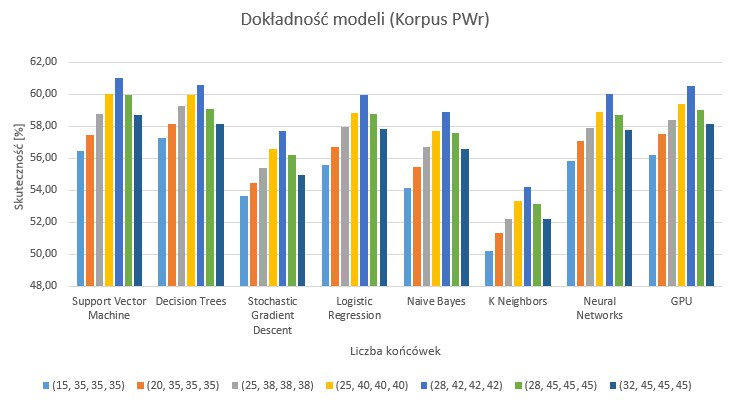
\includegraphics[width=\linewidth]{korpuspwrwykres}
	\label{Rysunek}
	\caption{Skuteczność modeli -- Korpus PWr}
\end{figure}

\begin{figure}[!htbp]
	\centering
	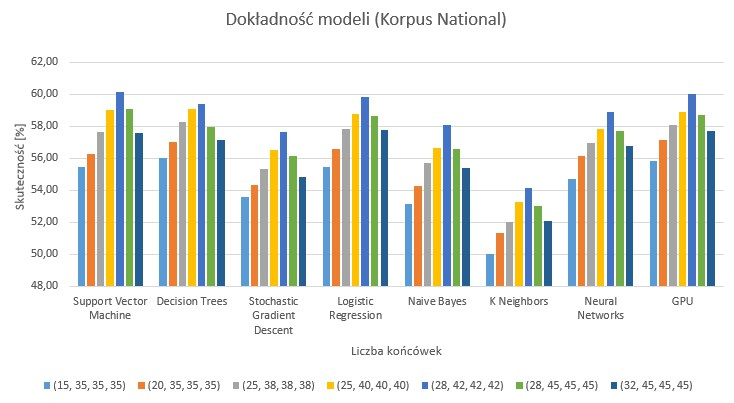
\includegraphics[width=\linewidth]{korpusnationalwykres}
	\label{Rysunek}
	\caption{Skuteczność modeli -- Korpus National}
\end{figure}


	
\end{document}